\documentclass{ctexart}
\usepackage{amsmath,amssymb,amsthm,bm}
\usepackage{xcolor}
\definecolor{Solarized-base03}{RGB}{0, 43, 54}
\definecolor{Solarized-base02}{RGB}{7, 54, 66}
\definecolor{Solarized-base01}{RGB}{88, 110, 117}
\definecolor{Solarized-base00}{RGB}{101, 123, 131}
\definecolor{Solarized-base0}{RGB}{131, 148, 150}
\definecolor{Solarized-base1}{RGB}{147, 161, 161}
\definecolor{Solarized-base2}{RGB}{238, 232, 213}
\definecolor{Solarized-base3}{RGB}{253, 246, 227}
\definecolor{Solarized-yellow}{RGB}{181, 137, 0}
\definecolor{Solarized-orange}{RGB}{203, 75, 22}
\definecolor{Solarized-red}{RGB}{220, 50, 47}
\definecolor{Solarized-magenta}{RGB}{211, 54, 130}
\definecolor{Solarized-violet}{RGB}{108, 113, 196}
\definecolor{Solarized-blue}{RGB}{38, 139, 210}
\definecolor{Solarized-cyan}{RGB}{42, 161, 152}
\definecolor{Solarized-green}{RGB}{133, 153, 0}
\color{Solarized-base01}
\pagecolor{Solarized-base3}

\newcommand{\red}[1]{\textcolor{Solarized-red}{#1}}
\newcommand{\yellow}[1]{\textcolor{Solarized-yellow}{#1}}
\newcommand{\blue}[1]{\textcolor{Solarized-blue}{#1}}
\newcommand{\cyan}[1]{\textcolor{Solarized-cyan}{#1}}
\newcommand{\violet}[1]{\textcolor{Solarized-violet}{#1}}

\usepackage{fullpage}
\usepackage{graphicx,epsfig,subfigure}
\usepackage{tikz,pgfplots}
\pgfplotsset{compat=1.17}
\usepackage{ifthen}
\usetikzlibrary{backgrounds,automata,shapes,snakes,arrows,arrows.meta,chains,positioning,calc}

%%%%%% 下面两行字体设置需根据自己的系统调整
\setmainfont[]{EBGaramond08-Regular}
\setCJKmainfont[BoldFont=FZHei-B01]{FZLongZhao-R-GB}
%%%%%%
\xeCJKsetup{CJKmath=true}
\everymath{\color{Solarized-magenta}}

\def \zerov {\bm{0}}
\def \av {\bm{a}}
\def \bv {\bm{b}}
\def \cv {\bm{c}}
\def \dv {\bm{d}}
\def \ev {\bm{e}}
\def \fv {\bm{f}}
\def \gv {\bm{g}}
\def \hv {\bm{h}}
\def \pv {\bm{p}}
\def \tv {\bm{t}}
\def \uv {\bm{u}}
\def \vv {\bm{v}}
\def \wv {\bm{w}}
\def \xv {\bm{x}}
\def \yv {\bm{y}}
\def \zv {\bm{z}}

\def \Av {\mathbf{A}}
\def \Bv {\mathbf{B}}
\def \Cv {\mathbf{C}}
\def \Dv {\mathbf{D}}
\def \Fv {\mathbf{F}}
\def \Gv {\mathbf{G}}
\def \Hv {\mathbf{H}}
\def \Iv {\mathbf{I}}
\def \Kv {\mathbf{K}}
\def \Lv {\mathbf{L}}
\def \Mv {\mathbf{M}}
\def \Pv {\mathbf{P}}
\def \Qv {\mathbf{Q}}
\def \Sv {\mathbf{S}}
\def \Uv {\mathbf{U}}
\def \Vv {\mathbf{V}}
\def \Wv {\mathbf{W}}
\def \Xv {\mathbf{X}}
\def \Yv {\mathbf{Y}}
\def \Zv {\mathbf{Z}}

\def \alphav {\bm{\alpha}}
\def \betav {\bm{\beta}}
\def \gammav {\bm{\gamma}}
\def \lambdav {\bm{\lambda}}
\def \Lambdav {\bm{\Lambda}}
\def \thetav {\bm{\theta}}
\def \epsilonv {\bm{\epsilon}}
\def \xiv {\bm{\xi}}
\def \muv {\bm{\mu}}
\def \Sigmav {\bm{\Sigma}}
\def \Phiv {\bm{\Phi}}
\def \nuv {\bm{\nu}}

\def \Acal {\mathcal{A}}
\def \Bcal {\mathcal{B}}
\def \Ical {\mathcal{I}}
\def \Lcal {\mathcal{L}}
\def \Ncal {\mathcal{N}}
\def \Pcal {\mathcal{P}}

\def \Dbb {\mathbb{D}}
\def \Ebb {\mathbb{E}}
\def \Nbb {\mathbb{N}}
\def \Qbb {\mathbb{Q}}
\def \Rbb {\mathbb{R}}
\def \Sbb {\mathbb{S}}

\def \Ifrak {\mathfrak{I}}
\def \Lfrak {\mathfrak{L}}
\def \Pfrak {\mathfrak{P}}

\def \diag {\mathrm{diag}}
\def \sign {\mathrm{sign}}
\def \sp {\mathrm{span}}
\def \diff {\mathrm{d}}
\def \tr {\mathrm{tr}}
\def \KL {\mathrm{KL}}
\def \var {\mathrm{var}}
\def \cov {\mathrm{cov}}
\def \ow {\mathrm{o.w.}}

\def \st {\mbox{s.t.}}
\def \const {\mbox{const}}

\DeclareMathOperator*{\argmin}{argmin}
\DeclareMathOperator*{\argmax}{argmax}

\allowdisplaybreaks[4]

\begin{document}
\title{}
\author{}
\date{}
\maketitle

\begin{figure}[ht]
    \centering

    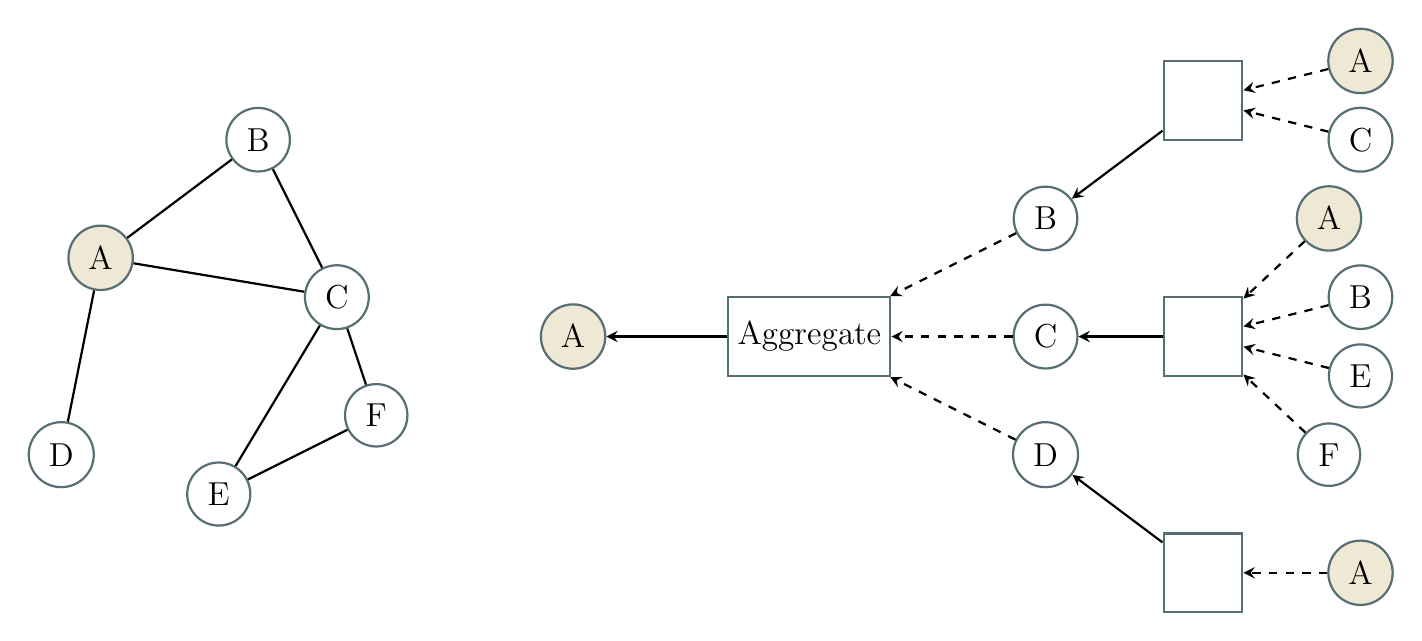
\begin{tikzpicture} [ % 先定义每类点的样式
            thick, >=stealth, scale=1, font=\large,
            rec/.style = {rectangle,minimum height = 1cm, minimum width = 2cm,draw=Solarized-base01},
            rec2/.style = {rectangle,minimum height = 1cm, minimum width = 1cm, draw=Solarized-base01},
            rec3/.style = {rectangle},
            point/.style = {circle, inner sep=4.0pt, draw=Solarized-base01},
            point-target/.style = {point, fill=Solarized-base2}
        ]

        % \draw [help lines, step = 1] (-10,-10) grid (10,10);
        % \filldraw (0,0) circle (0.1);

        % 中间矩形
        \node [rec] (r) at (-0.5,0) {Aggregate};
        \node [point-target] (pla1) at (-3.5,0) {A};

        % 右边点
        \node [point-target] (pra1) at (6.5,3.5) {A};
        \node [point] (prc1) at (6.5,2.5) {C};
        \node [point-target] (pra2) at (6.1,1.5) {A};
        \node [point] (prb1) at (6.5,0.5) {B};
        \node [point] (pre1) at (6.5,-0.5) {E};
        \node [point] (prf1) at (6.1,-1.5) {F};
        \node [point-target] (pra3) at (6.5,-3) {A};

        % 右边中间
        \node [point] (prcb) at (2.5,1.5) {B};
        \node [point] (prcc) at (2.5,0) {C};
        \node [point] (prcd) at (2.5,-1.5) {D};

        % 正方形
        \node [rec2] (rr1) at (4.5,3) {};
        \node [rec2] (rr2) at (4.5,0) {};
        \node [rec2] (rr3) at (4.5,-3) {};

        % 左边点
        \node [point] (plf) at (-6,-1) {F};
        \node [point] (plc) at (-6.5,0.5) {C};
        \node [point] (plb) at (-7.5,2.5) {B};
        \node [point-target] (pla) at (-9.5,1) {A};
        \node [point] (pld) at (-10,-1.5) {D};
        \node [point] (ple) at (-8,-2) {E};

        % 连线
        \draw (pla) -- (plb) -- (plc) -- (plf) -- (ple) -- (plc) -- (pla) -- (pld);

        \draw [->] (r) -- (pla1);
        \draw [->] (rr1) -- (prcb);
        \draw [->] (rr2) -- (prcc);
        \draw [->] (rr3) -- (prcd);

        \draw [dashed,->] (prcb) -- (r);
        \draw [dashed,->] (prcc) -- (r);
        \draw [dashed,->] (prcd) -- (r);

        \draw [dashed,->] (pra1) -- (rr1);
        \draw [dashed,->] (prc1) -- (rr1);

        \draw [dashed,->] (pra2) -- (rr2);
        \draw [dashed,->] (prb1) -- (rr2);
        \draw [dashed,->] (pre1) -- (rr2);
        \draw [dashed,->] (prf1) -- (rr2);

        \draw [dashed,->] (pra3) -- (rr3);

    \end{tikzpicture}

    \caption{The node graph.}
\end{figure}


\end{document}
